\section{Practical Implications and Experiments}
\subsection{Outline}
\note{
\begin{itemize}
    \item Verify trajectories match: 2 examples
    \item Delta mostly constant for GD (Appendix)
    \item Cubic spline
    \item 3D plots showing PL vs CS
    \item Same initialization in function space with different initialization has very different dynamics
\end{itemize}
}

In this section we present experimental results illustrating lazy and non-lazy training as well as the robustness to noise arising from flat minima.

\subsection{Preventing Noise Overfitting}
In the over-parameterized regime, a full rank kernel matrix produces interpolatory solutions. In the presence of noisy data, these solutions may be undesirable. Since knots in high curvature regions move faster initially (\todo{better way of saying this}), we can fit features in the data by limiting the number of iterations. Figure~\ref{fig:early-stopping} demonstrates the result for both the tangent and adaptive kernels. 

% {figures/nonlazy-square-noise.png}
\begin{figure}
    \centering
    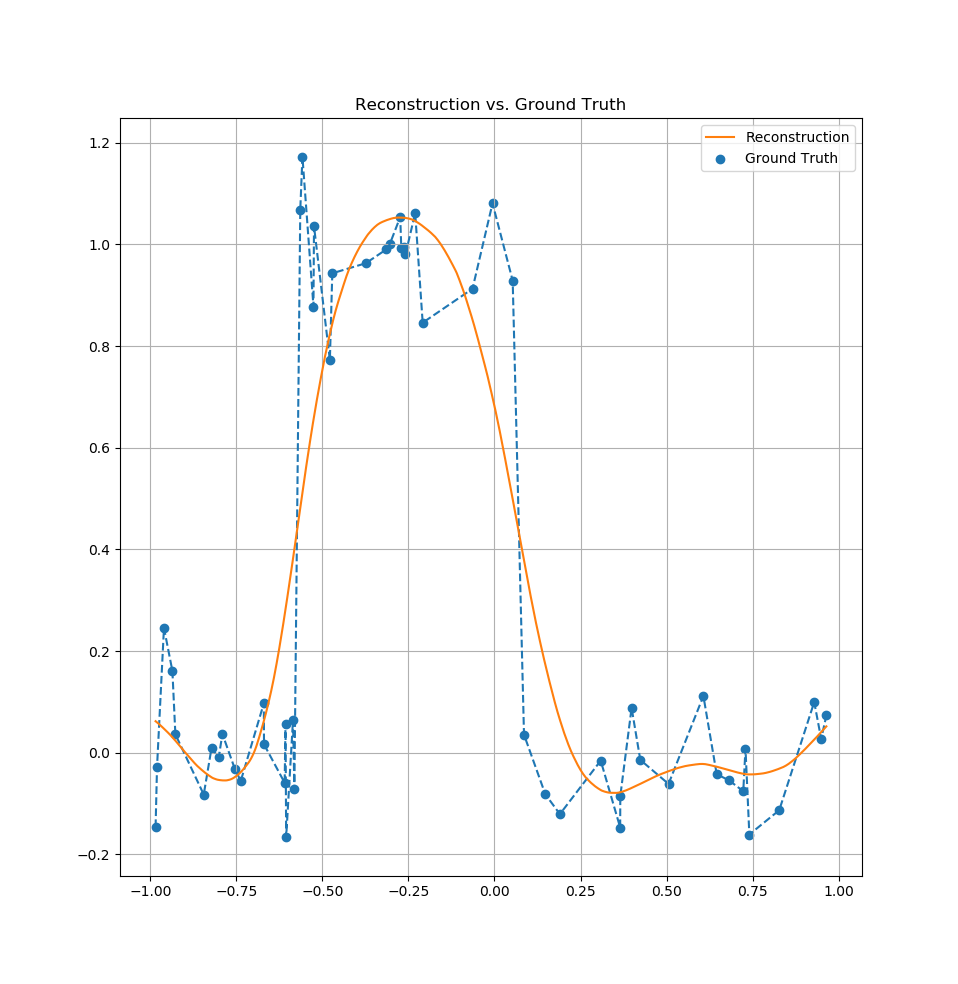
\includegraphics[width=0.45\textwidth]{figures/lazy-square-noise.png}
    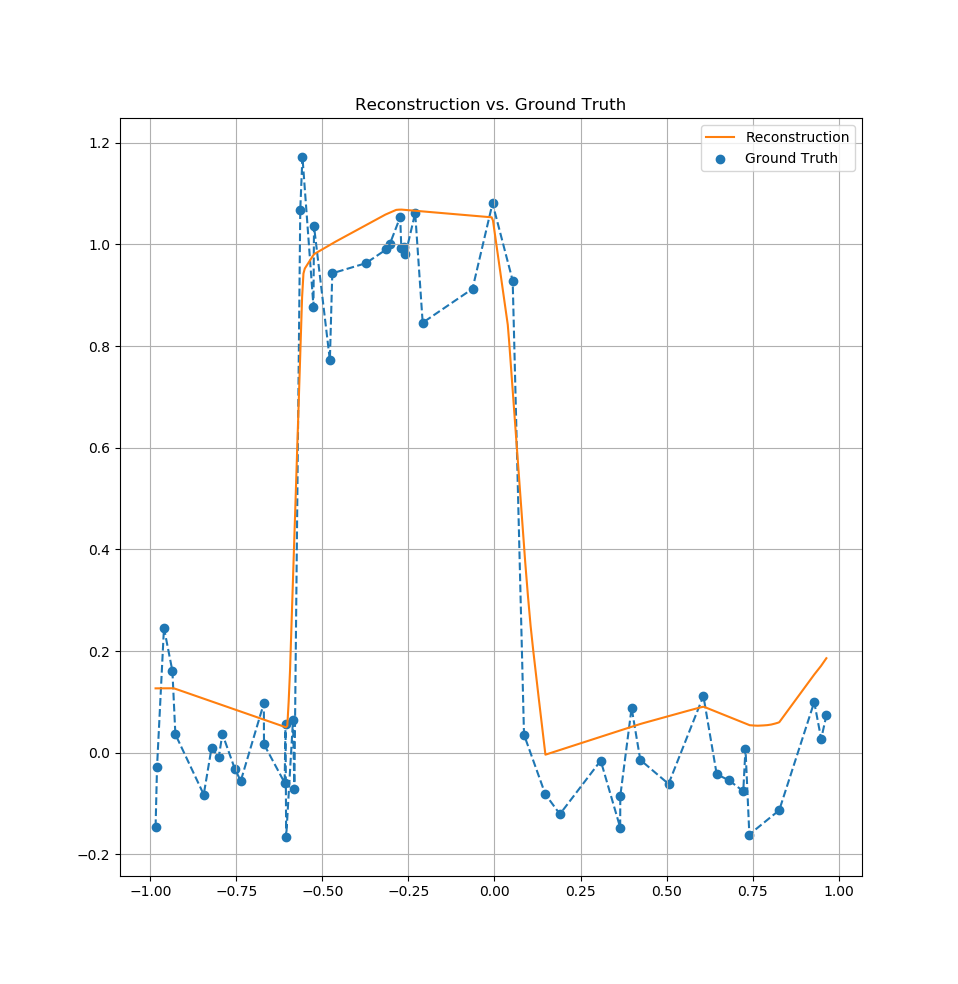
\includegraphics[width=0.45\textwidth]{figures/nonlazy-square-noise.png}
    \caption{The result of fitting a network with 2000 neurons to a square wave with gaussian noise added. Each network was fit with 10k iterations of gradient descent with Nesterov momentum. The left image shows the lazy training regime and the right shows the adaptive kernel regime.}
    \label{fig:early-stopping}
\end{figure}

Note however, that for a fixed kernel, regularization of the least squares problem will yields results similar to gradient descent with early stopping.

A natural consequence of considering only the dynamics of the kernel during training is that once a kernel has been fixed, we can control the smoothness and interpolation of the solution by tuning a single parameter and solving a linear system. We can thus control the quality of the model without retraining the network. 

Figure~\ref{fig:lsq-lazy} shows the result of varying regularization using the tangent kernel and Figure~\ref{fig:lsq-non-lazy} shows the result of regularization using the adaptive kernel.


\begin{figure}
    \centering
    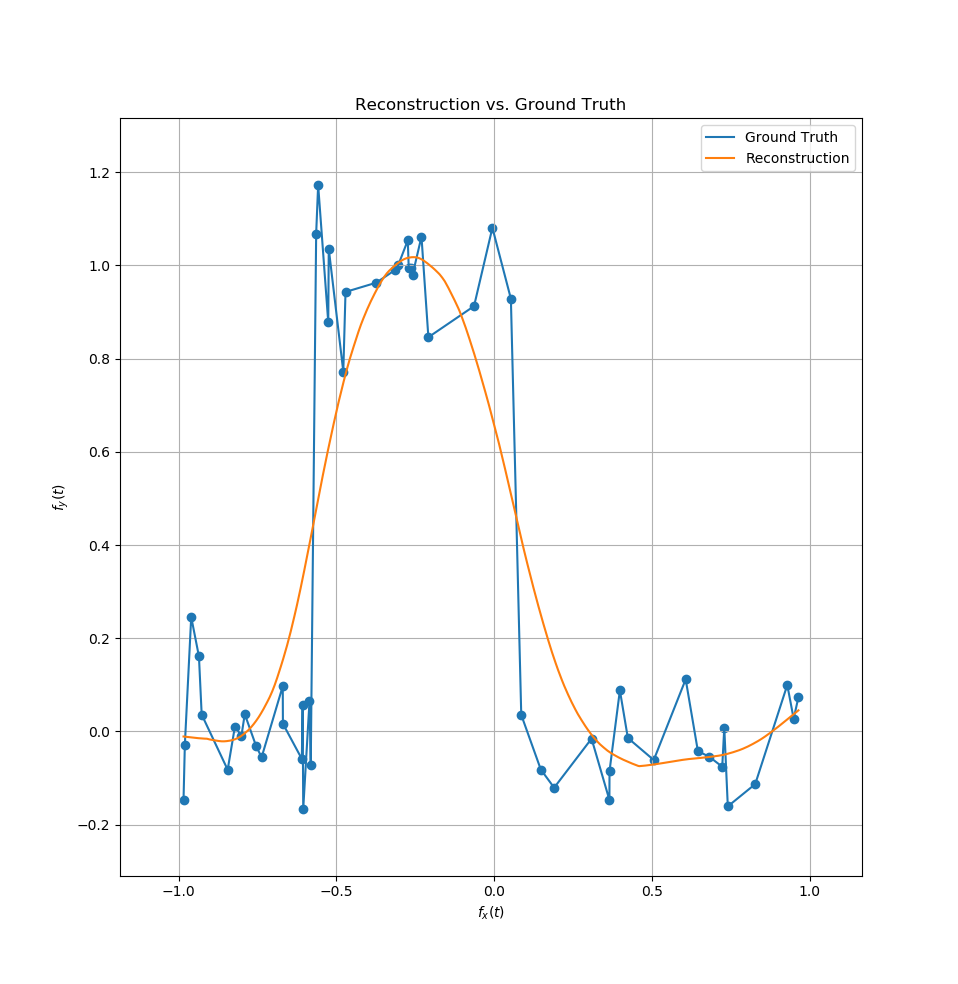
\includegraphics[width=0.32\textwidth]{figures/lazy-square-noise-lsq-1e0.png}
    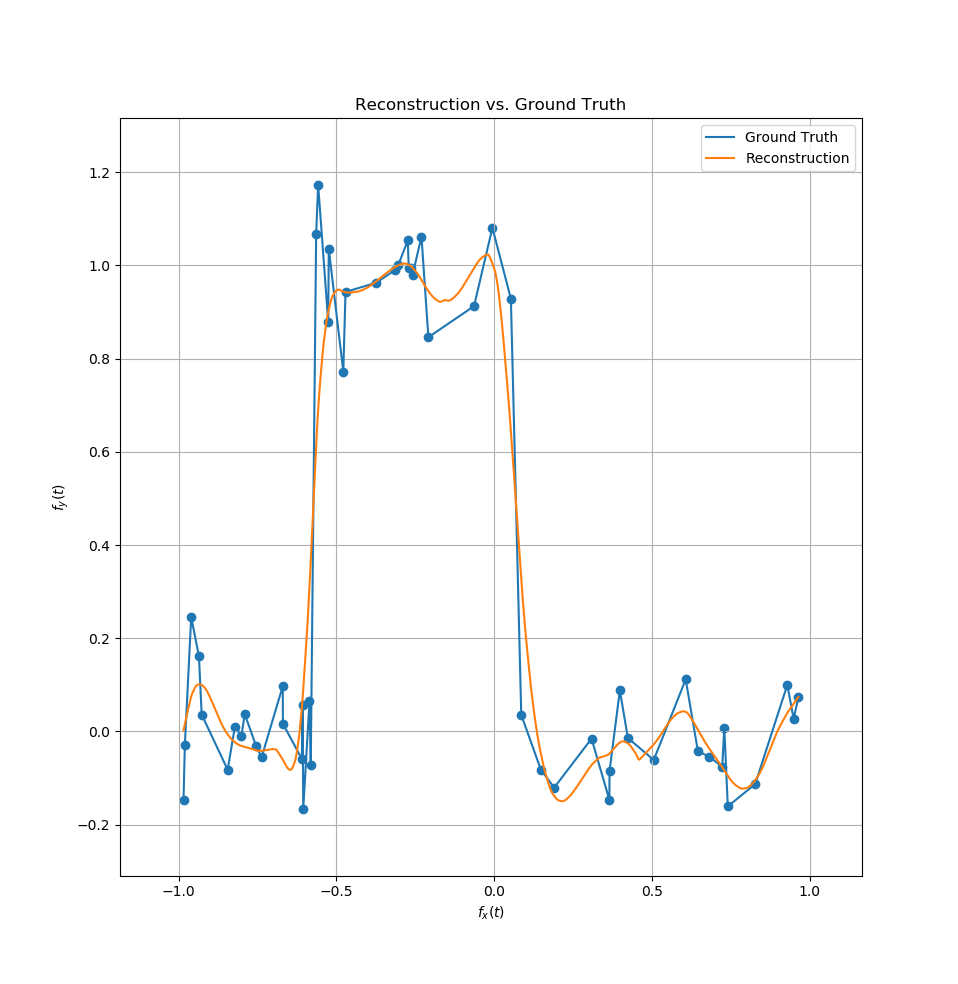
\includegraphics[width=0.32\textwidth]{figures/lazy-square-noise-lsq-1e-1.png}
    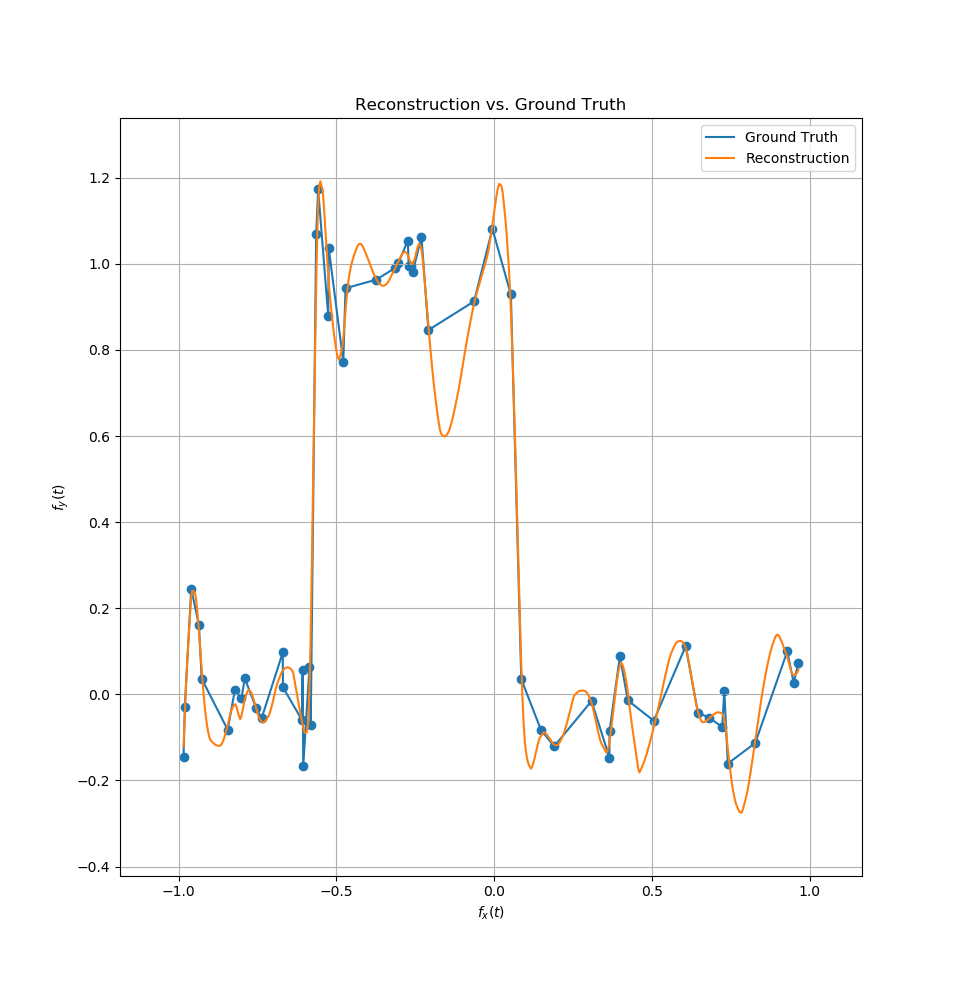
\includegraphics[width=0.32\textwidth]{figures/lazy-square-noise-lsq-1e-2.png}
    \caption{Regularized least squares kernel regression for the lazy kernel. We use different regularization factors (left: 1, mid: 0.1, right: 0.01) to control the smoothness of the solution.}
    \label{fig:lsq-lazy}
\end{figure}


\begin{figure}
    \centering
    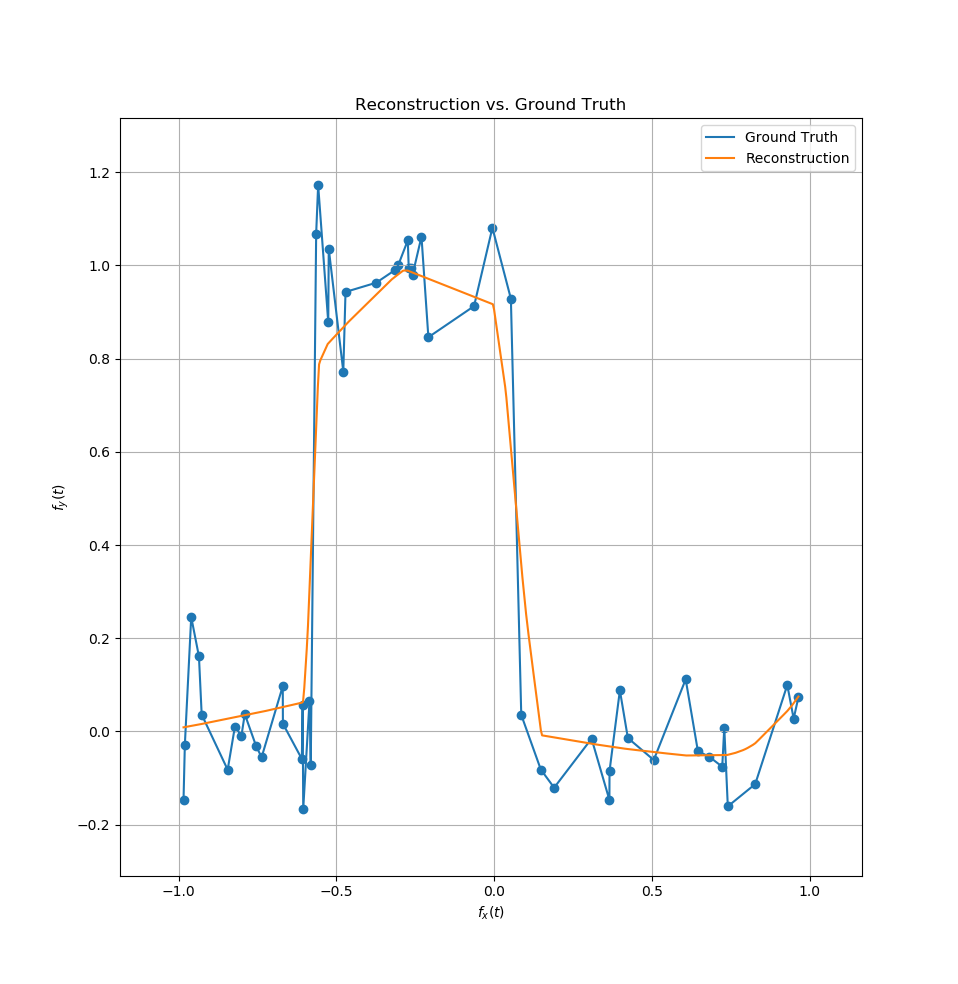
\includegraphics[width=0.32\textwidth]{figures/nonlazy-square-noise-lsq-1e0.png}
    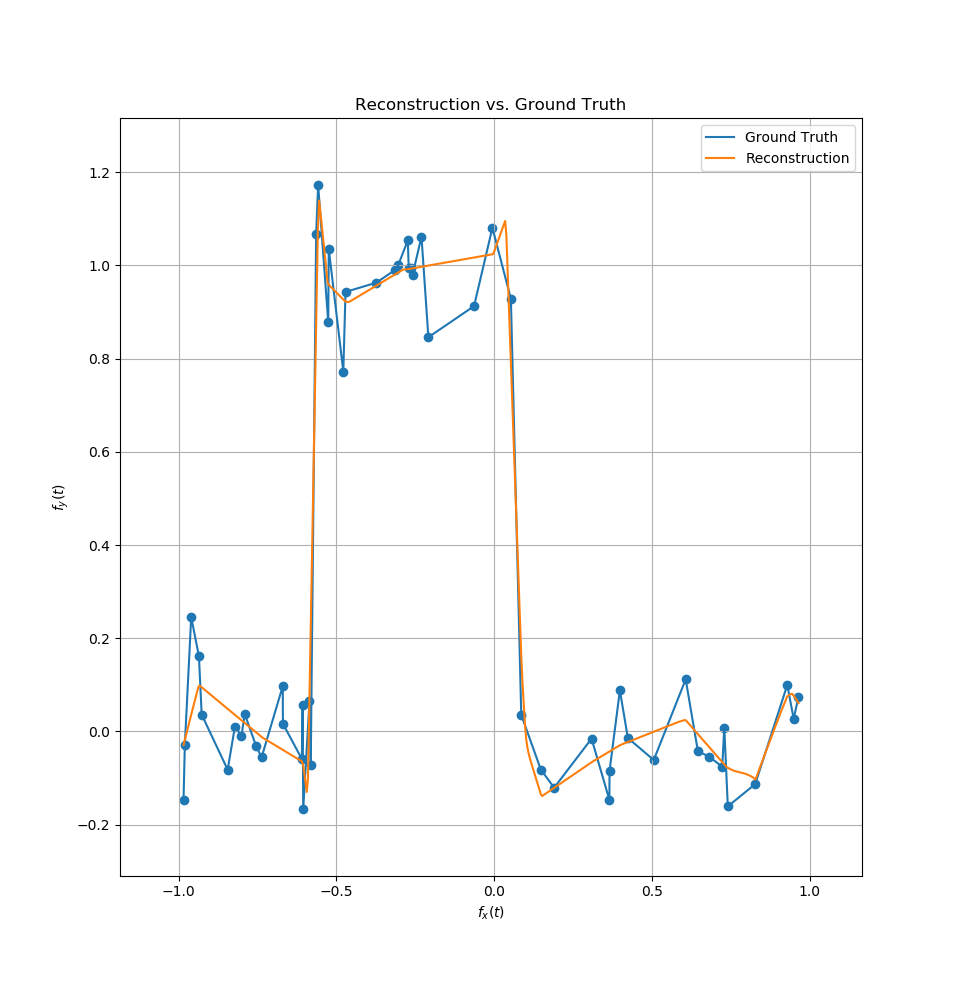
\includegraphics[width=0.32\textwidth]{figures/nonlazy-square-noise-lsq-1e-1.png}
    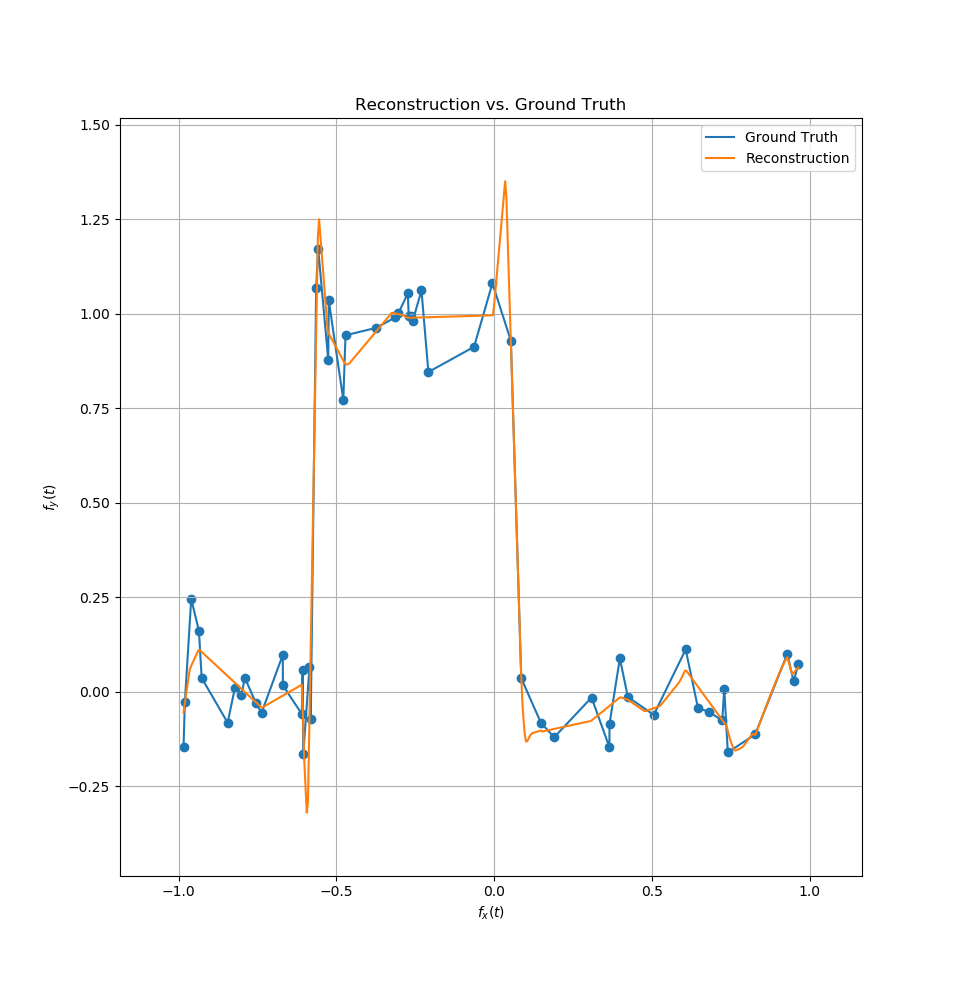
\includegraphics[width=0.32\textwidth]{figures/nonlazy-square-noise-lsq-1e-2.png}
    \caption{Regularized least squares kernel regression for the non-lazy kernel. We use different regularization factors (left: 1, mid: 0.1, right: 0.01) to controll the smoothness of the solution.}
    \label{fig:lsq-non-lazy}
\end{figure}